
\section{Introduction}

\begin{figure}[tb]
  \centering
  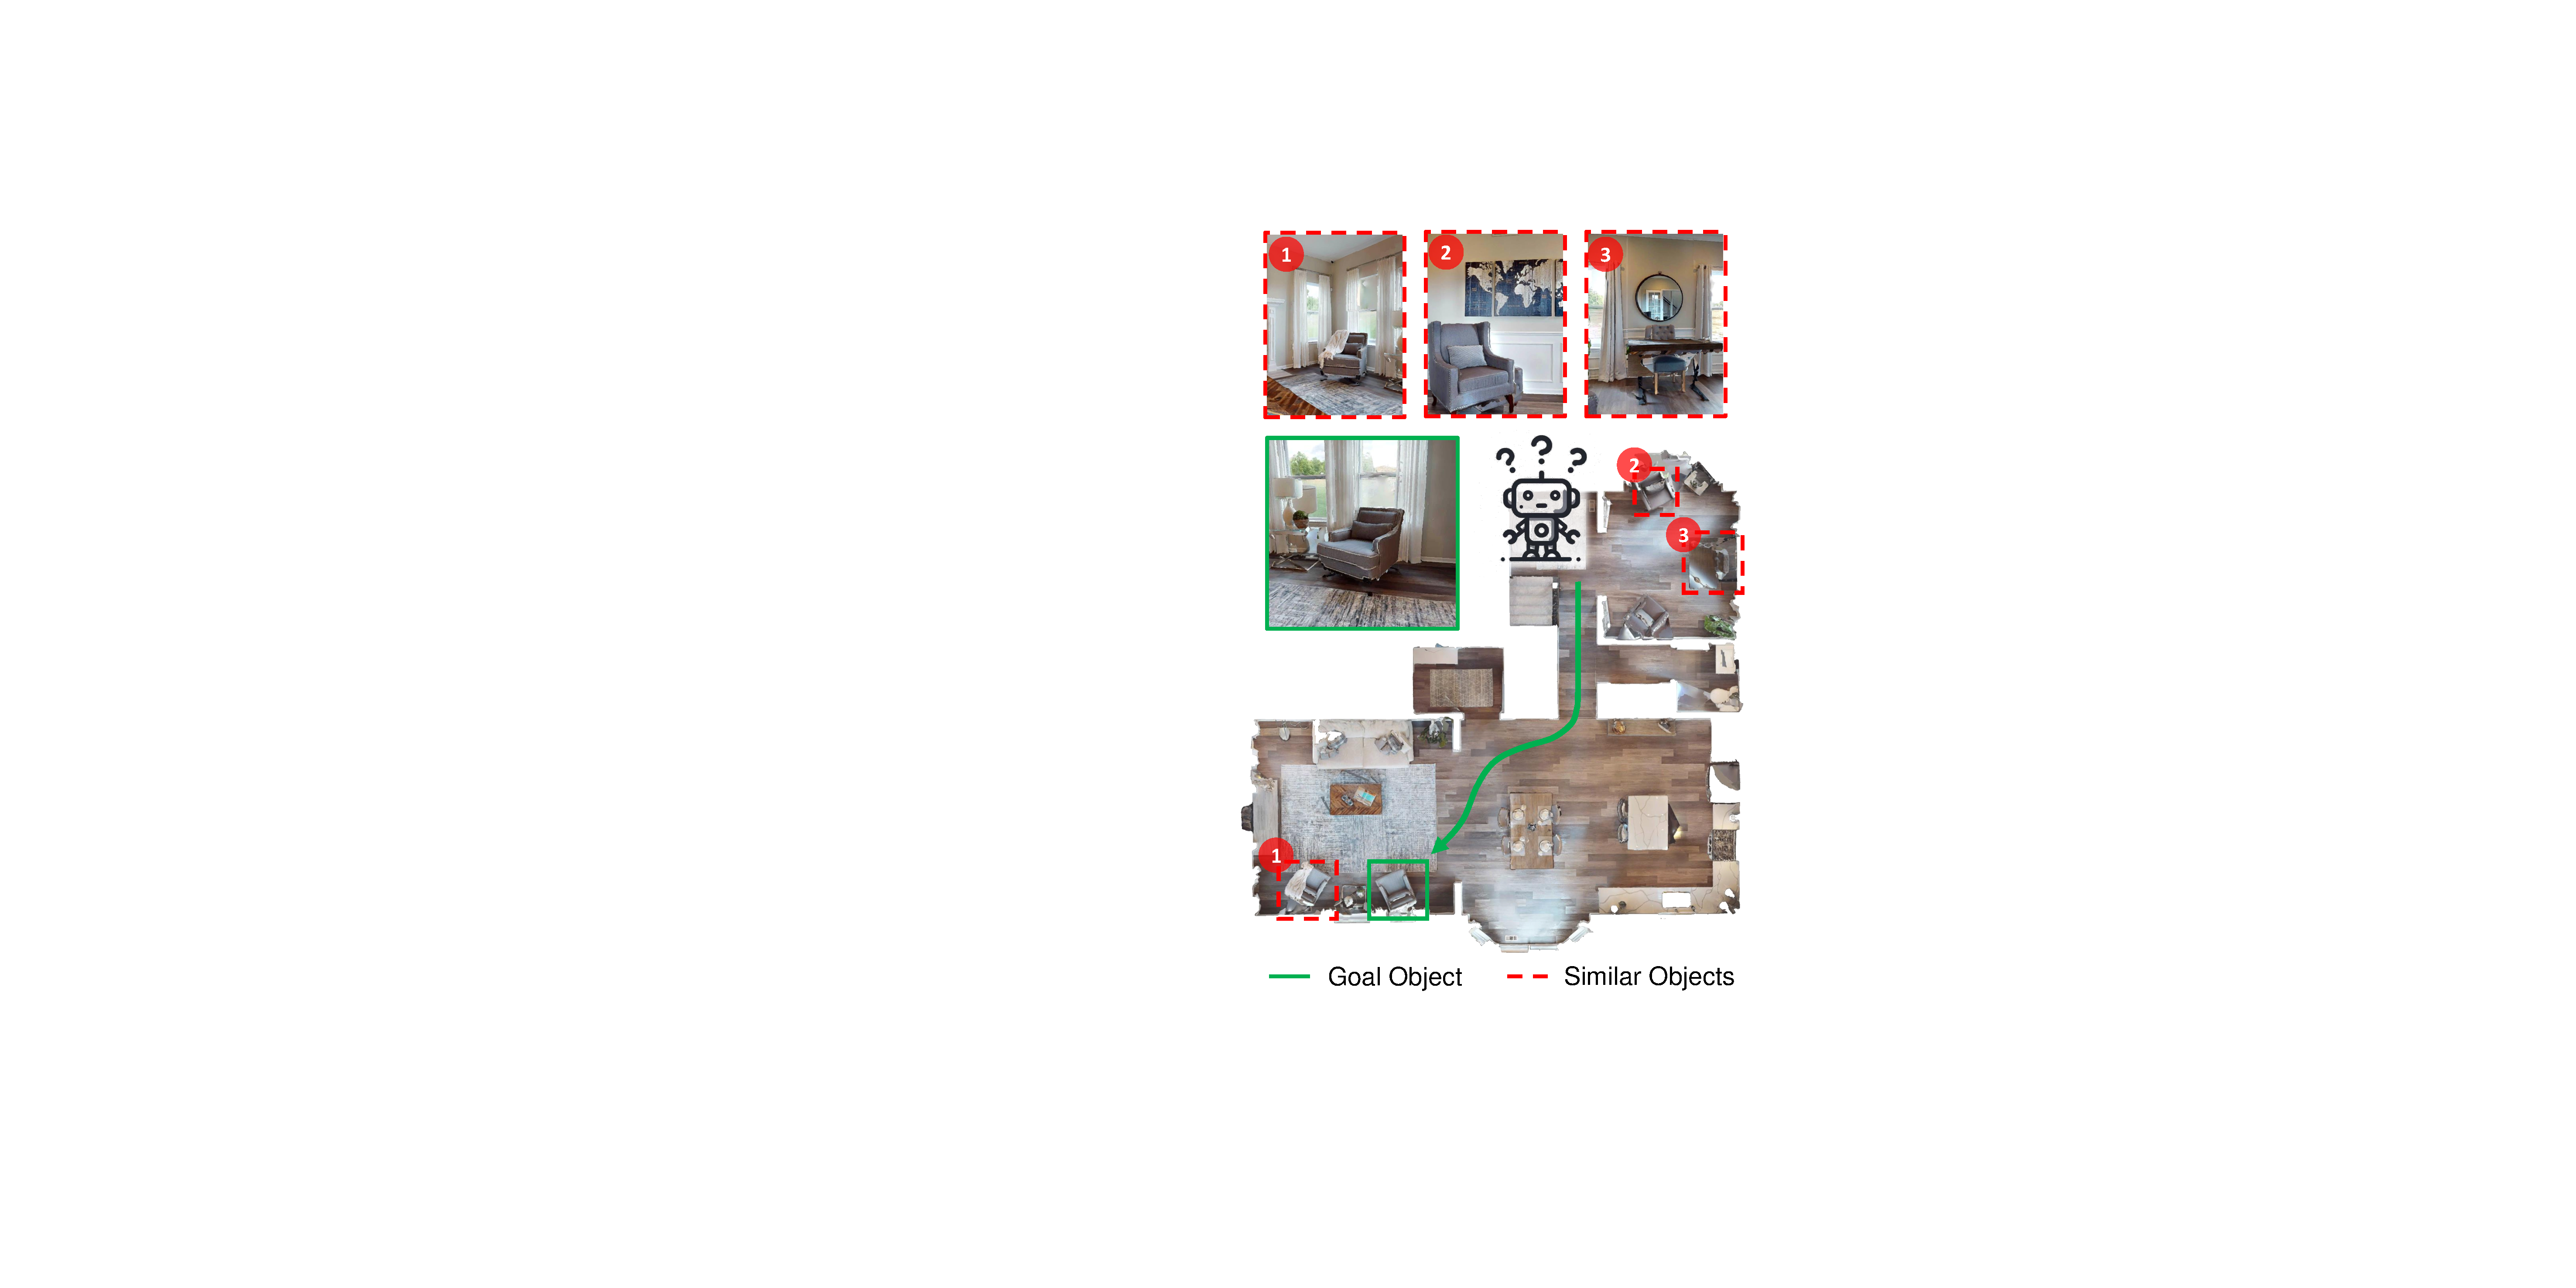
\includegraphics[width=0.9\linewidth]{pics/intro.pdf}
  \caption{Illustration of Instance ImageGoal Navigation (IIN), which requires agent to navigate to the object instance depicted in the goal image, while distinguishing it from other visually similar instances. 
  }
  \vspace{-16pt}
  \label{fig:intro}
\end{figure}


\IEEEPARstart{E}{mbodied} visual navigation is an emerging computer vision problem where an agent uses visual sensing to actively interact with the world and perform navigation tasks \cite{cheng2022learning, krantz2022sim, zhang2022generative, lin2022multimodal, qiao2023hop+, cai2021pose, lin2021adversarial, an2024etpnav, wu2023human, wang2020vision, wang2023learning, wang2022towards}. Recent years have witnessed substantial progress in embodied visual navigation, fueled by the availability of large-scale photo-realistic 3D scene datasets \cite{xia2018gibson, yadav2023habitat, chang2017matterport3d} and fast simulators for embodied navigation \cite{szot2022habitat, kolve2017ai2, savva2019habitat}. These advancements have enabled researchers to develop and test navigation algorithms in controlled environments that closely mimic real-world conditions. 

In embodied visual navigation, one critical question is ``how can we describe the goal target''.  One common setting for tasking an agent is to give it natural language instructions, such as ``check if my laptop is on the chair". However, this setting becomes confusing when there are multiple chairs in the house. To overcome this challenge, Krantz~\etal \cite{krantz2022instancespecific} propose Instance ImageGoal Navigation (IIN) \cite{krantz2023navigating, bono2023endtoend, lei2024instanceaware}. In IIN, an agent is presented with an image of a specific object, and its goal is to navigate to the specific object within the least time budget. The goal image is not expected to match the sensor specification or embodiment of the navigating agent, as described in \Cref{fig:intro}. To accomplish the task, the agent needs to distinguish the target object from different angle of views and ignore potential distractors. This is a challenging task as it involves semantic reasoning, geometry understanding and instance-aware matching.

To address the above issue, previous methods \cite{chaplot2020learning, chaplot2020object, krantz2023navigating, ramakrishnan2022poni, al2022zero, ma2022end, lei2024instanceaware} introduce 2D Semantic Bird-Eye-View (BEV) map to tackle this problem. These well-designed explicit map representations are memory-efficient, storing essential information such as 2D geometry and semantics, and can be directly utilized to calculate the agent's subsequent actions. However, this simple 2D BEV map representation lacks the capacity to retain 3D geometrical information about the environment, rendering it ineffective for navigating cross-floor scenarios. Additionally, BEV maps are unable to preserve the instance-aware features in a scene, which can be crucial for distinguishing between multiple objects of the same class or for tasks requiring fine-grained object interaction. 

% This leads to the inquiry: can we formulate a unified map representation for embodied agents to tackle the visual navigation problem?

To avoid the limitation of BEV maps, we propose a new Gaussian Splatting Navigation framework, \textit{i.e.}, GaussNav, for IIN task. Our GaussNav is inspired by the recent advancements in 3D Vision technologies, including Neural Radiance Fields (NeRF) \cite{mildenhall2020nerf} and 3D Gaussian Splatting (3DGS) \cite{kerbl3Dgaussians}. These technologies have demonstrated substantial progress in novel view synthesis (NVS) and 3D scene understanding. Although these technologies were not initially developed for navigation tasks, they offer considerable potential for application in this domain. To this end, we develop the Semantic Gaussian map representation, which integrates the representation of geometry, semantics and instance-aware features, and can be directly used for visual navigation. 

Our GaussNav framework consists of three stages, including Frontier Exploration, Semantic Gaussian Construction and Gaussian Navigation. 
First, the agent employs Frontier Exploration to collect observations of the unknown environment.
Second, the collected observations are used to construct Semantic Gaussian. By leveraging semantic segmentation algorithms \cite{he2017mask, wang2023internimage}, we assign semantic labels to each Gaussian. We then cluster Gaussians with their semantic labels and 3D positions, segmenting objects in the scene into different instances under various semantic categories. This representation is capable of preserving not only the 3D geometry of the scene and the semantic labels of each Gaussian, but also the texture details of the scene, thereby enabling NVS. 
Third, we render descriptive images for object instances, matching them with the goal image to effectively locate the target object. Upon determining the predicted goal object's position, we can efficiently transform our Semantic Gaussian into grid map and employ path planning algorithms to accomplish the navigation. 

To the best of our knowledge, we are the first to introduce 3DGS \cite{kerbl3Dgaussians} to embodied visual navigation. In this work, we unify the map representation of geometry, semantics and instance-aware features for visual navigation. Our framework can directly ground the target object with a single goal image input and guide the agent towards it without any additional exploration or verification \cite{lei2024instanceaware}. Our framework designs are beneficial for effective and efficient visual navigation. We evaluate our method's on both efficacy and efficiency and establish new state-of-the-art records on the challenging Habitat-Matterport 3D dataset (HM3D) \cite{yadav2023habitat}.





% \IEEEPARstart{E}{mbodied} Artificial Intelligence (EAI) is rapidly gaining traction as a prominent research domain. EAI focuses on developing agents capable of exploring, learning, reasoning, and interacting within the physical world. A fundamental challenge in this field is determining how an embodied agent can effectively comprehend its surrounding environment. One promising avenue for addressing this challenge is through the application of 3D Vision technologies, which significantly enhance environmental perception.

% Recent advancements in 3D Vision, such as Neural Radiance Fields (NeRF) \cite{mildenhall2020nerf} and 3D Gaussian Splatting (3DGS) \cite{kerbl3Dgaussians}, have demonstrated substantial progress in novel view synthesis and 3D scene understanding. Although these technologies were not initially developed with EAI tasks in mind, they offer considerable potential for application in this domain. This leads to a critical inquiry: how can we adapt and integrate these 3D Vision technologies to facilitate embodied tasks for agents? Exploring this question may unlock new capabilities for EAI systems, enhancing their ability to perceive and interact with complex physical environments.

% In this article, we focus on the embodied visual navigation \cite{cheng2022learning, krantz2022sim, zhang2022generative, lin2022multimodal, qiao2023hop+, cai2021pose, lin2021adversarial, an2024etpnav, wu2023human, wang2020vision, wang2023learning}, which studies the problem of navigating the embodied agent to desired location given semantic label or image input. This task definition requires the agent to effectively perceive and interpret visual information to navigate through its environment.

% \IEEEPARstart{A}{s} an emerging research topic, Embodied Artificial Intelligence (EAI) has been drawing an increasing interest in the community. 
% In EAI, the agents are expected to be capable of exploring, learning, reasoning, and interacting within the physical world. 
% A critical question then arises: how can an embodied agent comprehend the surrounding environment in the world? 
% One promising approach involves leveraging 3D Vision technologies to enhance environmental perception.
% Recent 3D Vision advancements, including Neural Radiance Fields (NeRF) \cite{mildenhall2020nerf} and 3D Gaussian Splatting (3DGS) \cite{kerbl3Dgaussians}, produce promising results in novel view synthesis and 3D scene understanding. These technologies are not originally designed for EAI tasks. So, this leads to the subsequent inquiry: how can we leverage these radian field technologies to facilitate embodied tasks for agents?

% This comprehension is especially crucial in the context of Embodied Visual Navigation, where an agent must effectively perceive and interpret visual information to navigate through its environment.
% To this end, many researchers resort to building different scene representations, including 2D Bird-Eye-View (BEV) map \cite{chaplot2020learning, chaplot2020object, krantz2023navigating, ramakrishnan2022poni, al2022zero, ma2022end}, 3D voxel grid \cite{chaplot2021seal, zhang20233d, tan2024self, trabucco2022simple}, Signed Distance Field (SDF) \cite{lu2019laser, reijgwart2019voxgraph, oleynikova2016signed, long2021learning}, etc..
% These map representations can well express the environment's geometry but lack the ability to retain the visual textures or object's features in the fine-level.

% Recent years have also witnessed rapid advancements in radian field technologies, exemplified by the development of Neural Radiance Fields (NeRF) \cite{mildenhall2020nerf} and 3D Gaussian Splatting (3DGS) \cite{kerbl3Dgaussians}, among others. 
% This leads to the subsequent inquiry: how can we leverage these radian field technologies to facilitate embodied tasks for agents?

% Based on the above motivation, we focus on the embodied visual navigation \cite{cheng2022learning, krantz2022sim, zhang2022generative, lin2022multimodal, qiao2023hop+, cai2021pose, lin2021adversarial, an2024etpnav, wu2023human, wang2020vision, wang2023learning}. Traditional navigation research addresses point-to-point navigation, a problem extensively studied in past years. However, the advent of deep learning technologies has reignited interest in navigating agents and comprehending the semantic intricacies of 3D environments. For instance, consider a scenario where an agent is presented with a randomly captured image of a specific object, the agent's task is to navigate to this object within a certain time budget. To distinguish the target from different angle of views, the agent has to understand the object's geometry, its semantic attributes, and its spatial relationship to the environment. This task, named as Instance ImageGoal Navigation (IIN) was introduced by Krantz \etal \cite{krantz2022instancespecific} for embodied visual navigation, as depicted in \Cref{fig:intro}.

% Recently, map-based visual navigation methods \cite{chaplot2020learning, chaplot2020object, krantz2023navigating, ramakrishnan2022poni, al2022zero, ma2022end} have focused on constructing explicit episodic Bird-Eye-View (BEV) maps, achieving notable success in established visual navigation benchmarks. These well-designed explicit map representations are memory-efficient, storing essential information such as 2D geometry and semantics, and can be directly utilized to calculate the agent's subsequent actions. However, this simple 2D BEV map representation is not free from its limitations. For instance, it lacks the capacity to retain 3D geometrical information about the environment, rendering it ineffective for navigating cross-floor scenarios. Additionally, BEV maps are unable to preserve the intricate textures and detailed features in a scene. To address the above issues in existing map-based visual navigation methods, we propose a new Gaussian Splatting Navigation framework, \textit{i.e.}, GaussNav, for IIN task.


% Our GaussNav framework consists of three stages, including sub-Gaussians Division, Semantic Gaussian Construction and Gaussian Navigation. 
% First, to address the optimization difficulties of 3DGS in large scenes on computationally constrained devices, we propose to divide Gaussians into corresponding sub-Gaussians and to optimize each of them individually. 
% Second, we introduce a new form of map representation, \textit{i.e.}, Semantic Gaussian. By leveraging semantic segmentation algorithms \cite{he2017mask, wang2023internimage}, we assign semantic labels to each Gaussian. We then cluster Gaussians with their semantic labels and 3D positions, segmenting objects in the scene into different instances under various semantic categories. This representation is capable of preserving not only the 3D geometry of the scene and the semantic labels of each Gaussian but also the texture details of the scene, thereby enabling novel view synthesis. 
% Third, we render descriptive images for object instances, matching them with the goal image to effectively locate the target object. Upon determining the predicted goal object's position, we can efficiently transform our Semantic Gaussian into grid map and employ path planning algorithms. To the best of our knowledge, we are the first to introduce 3DGS \cite{kerbl3Dgaussians} to embodied visual navigation. We evaluate our method's on both efficacy and efficiency and establish new state-of-the-art records on the challenging Habitat-Matterport 3D dataset (HM3D) \cite{yadav2023habitat}.

% With our proposed method, GaussNav, the difficult IIN task can be transformed into a more tractable PointGoal Navigation task, consequently yielding more promising results. On the challenging Habitat-Matterport 3D dataset (HM3D) \cite{yadav2023habitat}, we achieve $0.725$ success and $0.578$ SPL. This represents a significant improvement over the previous state-of-the-art work \cite{lei2024instanceaware}, which reported success of $0.702$ and SPL of $0.252$.


